% Copyright (c) 2022 by Lars Spreng
% This work is licensed under the Creative Commons Attribution 4.0 International License. 
% To view a copy of this license, visit http://creativecommons.org/licenses/by/4.0/ or send a letter to Creative Commons, PO Box 1866, Mountain View, CA 94042, USA.

%~~~~~~~~~~~~~~~~~~~~~~~~~~~~~~~~~~~~~~~~~~~~~~~~~~~~~~~~~~~~~~~~~~~~~~~~~~~~~~
% You can add your packages and commands to the loadslides.tex file. 
% The files in the folder "styles" can be modified to change the layout and design of your slides.
% I have included examples on how to use the template below. 
% Some of these examples are taken from the Metropolis template.
%~~~~~~~~~~~~~~~~~~~~~~~~~~~~~~~~~~~~~~~~~~~~~~~~~~~~~~~~~~~~~~~~~~~~~~~~~~~~~~


\documentclass[
12pt,notheorems,hyperref={pdfauthor=whatever}
]{beamer}


% Copyright (c) 2022 by Lars Spreng
% This work is licensed under the Creative Commons Attribution 4.0 International License. 
% To view a copy of this license, visit http://creativecommons.org/licenses/by/4.0/ or send a letter to Creative Commons, PO Box 1866, Mountain View, CA 94042, USA.

%~~~~~~~~~~~~~~~~~~~~~~~~~~~~~~~~~~~~~~~~~~~~~~~~~~~~~~~~~~~~~~~~~~~~~~~~~~~~~~
% Add your packages and commands to this file
%~~~~~~~~~~~~~~~~~~~~~~~~~~~~~~~~~~~~~~~~~~~~~~~~~~~~~~~~~~~~~~~~~~~~~~~~~~~~~~

%~~~~~~~~~~~~~~~~~~~~~~~~~~~~~~~~~~~~~~~~~~~~~~~~~~~~~~~~~~~~~~~~~~~~~~~~~~~~~~
% Fonts
% \RequirePackage{palatino} % for serif slides
% \usefonttheme{serif}
\RequirePackage[scaled]{helvet} % for sans-serif slides

\RequirePackage[utf8]{inputenc}
\RequirePackage[T1]{fontenc}


\usepackage{styles/elegantmacros}
\usefolder{styles}
\usetheme[style=red]{elegant}

\newcommand{\makepart}[1]{ % For convenience
\part{#1} \frame{\partpage}
}

\usepackage{setspace}
\renewcommand{\baselinestretch}{1.125} 

%~~~~~~~~~~~~~~~~~~~~~~~~~~~~~~~~~~~~~~~~~~~~~~~~~~~~~~~~~~~~~~~~~~~~~~~~~~~~~~

%~~~~~~~~~~~~~~~~~~~~~~~~~~~~~~~~~~~~~~~~~~~~~~~~~~~~~~~~~~~~~~~~~~~~~~~~~~~~~~
% Figures
\RequirePackage{booktabs}
\RequirePackage{colortbl}
\RequirePackage{ragged2e}
\RequirePackage{schemabloc}
%\RequirePackage{natbib}
\RequirePackage{caption}
\RequirePackage{subcaption}
\RequirePackage{tabularx}
\RequirePackage{array}
\RequirePackage{multirow}
\RequirePackage[%
  natbib=true, backend=biber,%
  style=apa, isbn=false,url=false,uniquename=false%, useprefix=true%
  ]{biblatex}
\addbibresource{references.bib}
\newcolumntype{Y}{>{\centering\arraybackslash}X}

%~~~~~~~~~~~~~~~~~~~~~~~~~~~~~~~~~~~~~~~~~~~~~~~~~~~~~~~~~~~~~~~~~~~~~~~~~~~~~~

%~~~~~~~~~~~~~~~~~~~~~~~~~~~~~~~~~~~~~~~~~~~~~~~~~~~~~~~~~~~~~~~~~~~~~~~~~~~~~~
% Figures
\RequirePackage{wrapfig}
\RequirePackage{pgfplots}
\RequirePackage{graphicx}
\RequirePackage{adjustbox}
\RequirePackage{environ}
\pgfplotsset{compat=1.18}

\makeatletter
\newsavebox{\measure@tikzpicture}
\NewEnviron{scaletikzpicturetowidth}[1]{%
  \def\tikz@width{#1}%
  \def\tikzscale{1}\begin{lrbox}{\measure@tikzpicture}%
  \BODY
  \end{lrbox}%
  \pgfmathparse{#1/\wd\measure@tikzpicture}%
  \edef\tikzscale{\pgfmathresult}%
  \BODY
}
\makeatother
%~~~~~~~~~~~~~~~~~~~~~~~~~~~~~~~~~~~~~~~~~~~~~~~~~~~~~~~~~~~~~~~~~~~~~~~~~~~~~~

%~~~~~~~~~~~~~~~~~~~~~~~~~~~~~~~~~~~~~~~~~~~~~~~~~~~~~~~~~~~~~~~~~~~~~~~~~~~~~~
% Maths 
\RequirePackage{textcomp}
\RequirePackage{amsmath} 
\RequirePackage{amsthm}
\RequirePackage{mathtools}
%\RequirePackage{bbm}
%\RequirePackage{algorithm}
% \RequirePackage[osf,sc]{mathpazo}
%\RequirePackage{pifont}
%\newcommand{\xmark}{\ding{55}}%
%\numberwithin{equation}{section}
\DeclareMathOperator*{\argmax}{arg\,max}
\DeclareMathOperator*{\argmin}{arg\,min}

\setbeamertemplate{theorems}[numbered] % to number

\theoremstyle{definition}
\newtheorem{fact}{Fact}[section]
\newtheorem{examp}{Exemplo}[section]

\theoremstyle{plain}
\newtheorem{definition}{Definição}[section]
\newtheorem{proposition}{Proposição}
\newtheorem{theorem}{Teorema}
\newtheorem{cor}{Corolário}
\newtheorem{assumption}{Assumption}

\providecommand{\H}{\mathscr{H}}      
\providecommand{\E}{\mathbb{E}}
\makeatletter
\def\munderbar#1{\underline{\sbox\tw@{$#1$}\dp\tw@\z@\box\tw@}}
\makeatother

%~~~~~~~~~~~~~~~~~~~~~~~~~~~~~~~~~~~~~~~~~~~~~~~~~~~~~~~~~~~~~~~~~~~~~~~~~~~~~~

% Costumização
\usepackage{booktabs}
\usepackage{multirow}
\usepackage{makecell}
\usepackage{xparse}
\usepackage{xifthen}
\usepackage{xstring}
\usepackage{etoolbox} % needed for \IfEqCase
\usepackage{longtable}
\usetikzlibrary{patterns}
\usetikzlibrary{arrows.meta}

\addtobeamertemplate{title page}{
  \begin{tikzpicture}[remember picture,overlay]
    \node[anchor=south east,xshift=-1cm,yshift=0.5cm]
      at (current page.south east)
      {
\includegraphics[height=.5cm]{figures/pargo.png}};
  \end{tikzpicture}
}{}

\setbeamercolor{title}{bg=}
\setbeamercolor{author}{bg=}
\setbeamercolor{institute}{bg=}
\setbeamercolor{date}{bg=}

\definecolor{c0}{rgb}{1.00, 1.00, 1.00} % branco
\definecolor{c1}{rgb}{0.20, 0.40, 0.80} % azul
\definecolor{c2}{rgb}{0.90, 0.20, 0.10} % vermelho
\definecolor{c3}{rgb}{1.00, 0.60, 0.00} % amarelo
\definecolor{c4}{rgb}{0, 0.61, 0.29}
% 
\usetikzlibrary{positioning}
\usetikzlibrary{decorations.pathreplacing}
\usetikzlibrary{decorations.pathmorphing}
\usetikzlibrary{decorations}

\tikzstyle{every node}=[shape=circle, minimum size=.4em, inner sep=0.1em]
\tikzstyle{vertex}=[circle, draw=black, minimum size=0.4em, fill=black, inner sep=0.1em]
% \tikzstyle{label}=[fill=none]
\tikzstyle{positive}=[dashed]
\tikzset{parallel/.style={auto=right,
		to path={ let \p1=(\tikztostart),\p2=(\tikztotarget),
			\n1={atan2(\y2-\y1,\x2-\x1)},\n2={\n1+180}
			in ($(\tikztostart.{\n1})!.1em!270:(\tikztotarget.{\n2})$) -- 
			($(\tikztotarget.{\n2})!.1em!90:(\tikztostart.{\n1})$) \tikztonodes}}}
\tikzset{
  node_alert/.style={circle,draw, color=c3, line width=1.5pt, opacity=0.6, minimum size=13pt, scale=0.6, inner sep=0.5pt},
  alert_red/.style={circle,draw, color=c2, line width=1.5pt, opacity=0.6, minimum size=13pt, scale=0.6, inner sep=0.5pt},
  % label/.style={draw=none},
  edge/.style = {->, line width=0.02cm},
  edgeb/.style = {->, line width=0.05cm},
  edge1/.style = {rounded corners, c3, opacity=0.6, line width=3pt},
  edge2/.style = {rounded corners, c1, opacity=0.6, line width=3pt},
}
%%%% para fazer "animações"
\tikzset{
    invisible/.style={opacity=0,text opacity=0},
    visible on/.style={alt=#1{}{invisible}},
    alt/.code args={<#1>#2#3}{%
      \alt<#1>{\pgfkeysalso{#2}}{\pgfkeysalso{#3}} % \pgfkeysalso doesn't change the path
    },
}

\renewcommand{\figurename}{\footnotesize Fig}
\newtheorem{problem}{Problema}
\newtheorem{lemma}{Lema}
\newtheorem{prop}{Proposição}

\newcommand{\Problem}[3]{
	\begin{block}{{\scshape #1}}
		{\bfseries Entrada:} #2\\
		{\bfseries Objetivo:} #3
	\end{block}%
}

\newcommand{\fakepart}[1]{
  \section{}
  \begin{frame}
    \centering
    \vfill
    {\LARGE\emphasize{#1}}
    \vfill
  \end{frame}
}

\newcommand{\zero}{\mathbf{0}}
\newcommand{\Px}{\mathbf{P}}
\newcommand{\PxK}{\mathbf{P}(K)}
\newcommand{\Py}{\mathbf{P}'}

\newcommand{\R}{\mathbb{R}}
\newcommand{\PxG}{\mathbf{P}(G)}
\newcommand{\PG}{{\mathcal{P}_G}}
\newcommand{\PGn}{{\overline{\mathcal{P}}_G}}
\newcommand{\Cn}{{\mathcal{C}^-}}
\newcommand{\Tc}{\mathcal{T}}
\newcommand{\Cc}{\mathcal{C}}
\newcommand{\Z}{\mathbb{Z}}
\newcommand{\B}{\mathbb{B}}
\newcommand{\Q}{\mathbb{Q}}
\newcommand{\m}[1]{\mathbf{#1}}
\newcommand{\tr}{\mathrm{t}}
\newcommand{\cl}[1]{\mathcal{#1}}
\newcommand{\Mcl}{\m{\mathit{M}}}
\newcommand{\Mbcl}[1]{\m{\mathit{M}}(b(\cl{#1}))}
\newcommand{\lpp}[1]{\ensuremath{\mathrm{#1}}}
\newcommand{\cN}{\ensuremath{\mathcal{N}\!}}
\newcommand{\cV}{\ensuremath{\mathcal{V}\!}}
\newcommand{\tp}{{\top\!}}
\newcommand{\e}{\mathbf{e}}

\NewDocumentCommand{\Xvtx}{o m}{
  % #1 = optional hat (if present)
  % #2 = inner exponent (uvw)
  \IfNoValueTF{#1}
    {x^{{#2}}} % No accent
    {%
      \IfEqCase{#1}{
        {hat}{\hat{x}^{{#2}}}
        {bar}{\bar{x}^{{#2}}}
        {tilde}{\tilde{x}^{{#2}}}
        {dot}{\dot{x}^{{#2}}}
        {dots}{\ddot{x}^{{#2}}}
      }[\PackageError{nestedexp}{Unknown accent '#1'}{}]%
    }
}
\NewDocumentCommand{\Yvtx}{o m}{
  % #1 = optional hat (if present)
  % #2 = inner exponent (uvw)
  \IfNoValueTF{#1}
    {y^{{#2}}} % No accent
    {%
      \IfEqCase{#1}{
        {hat}{\hat{y}^{{#2}}}
        {bar}{\bar{y}^{{#2}}}
        {tilde}{\tilde{y}^{{#2}}}
        {dot}{\dot{y}^{{#2}}}
        {dots}{\ddot{y}^{{#2}}}
      }[\PackageError{nestedexp}{Unknown accent '#1'}{}]%
    }
} % Loads packages and some defined commands

\title[
   Problema do Subgrafo Gerador Balanceado Máximo:\\desigualdades válidas e estratégias de branch-and-cut
]{Problema do Subgrafo Gerador Balanceado Máximo:\\desigualdades válidas e estratégias de branch-and-cut}

\author[
% Text entered here will appear in the bottom left corner
]{
    Natália Coelho, Manoel Campêlo
}

\institute{
    Universidade Federal do Ceará}
\date{Julho, 2026}

\begin{document}

% Generate title page
{
\setbeamertemplate{footline}{} 
\begin{frame}[plain]
    \begin{tikzpicture}[remember picture,overlay]
    \node[
        opacity=0.1,
        inner sep=0pt
    ] at (current page.center)
    {
\includegraphics[width=0.9\paperwidth]{figures/capa-ufc.png}};
    \end{tikzpicture}

  \titlepage
\end{frame}
}
\addtocounter{framenumber}{-1}

% You can declare different parts as a parentof sections
% \begin{frame}[allowframebreaks]{Sumário}
%     \tableofcontents
% \end{frame}

\section{Introdução}

\subsection{Definições preliminares}
\begin{frame}[fragile]
	\begin{definition}[\cite{harary1953notion}]
		Um \textbf{grafo de sinais} é um grafo $G = (V, E, \sigma)$, em que $\sigma$ é uma função $\sigma: E \to \{+,-\}$.
	\end{definition}
	\begin{minipage}[h][12em][c]{\textwidth}
		\centering%
			\vspace{1em}
		  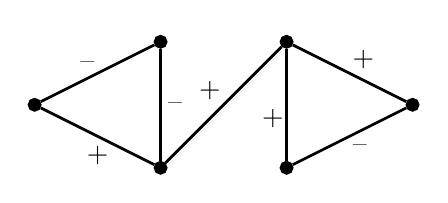
\begin{tikzpicture}[scale = 0.8]
    \pgfsetlinewidth{1pt}
    % \tikzset{vertex/.style={circle, fill=black, minimum size=0.8em, inner sep=0.1em}};


    \node[vertex] (c1) at (-3,0){};

    \node[vertex] (c2) at (-1,1){};

    \node[vertex] (c3) at (-1,-1){};

    \node[vertex] (c4) at (1,1){};

    \node[vertex] (c5) at (3,0){};

    \node[vertex] (c6) at (1,-1){};


	{
        \draw (c1) -- (c2) node [label, midway, above left] {--};
        \draw (c2) -- (c3) node [label, midway, right] {--};
        \draw (c3) -- (c1) node [label, midway, below] {+};
        
        \draw (c3) -- (c4) node [label, midway, above left] {+};
        
        \draw (c4) -- node [label, midway, above right] {+} (c5);
        \draw (c5) -- node [label, midway, below right] {--} (c6);
        \draw (c6) -- node [label, midway, below left] {+} (c4);
	}

	% \only<2->{
	% \draw (c1) edge[c2] node [label, midway, above left] {--} (c2);
	% \draw (c2) edge[c2] node [label, midway, right] {--} (c3);
	% \draw (c3) edge[c1]  node [label, midway, below] {+} (c1);

  %   \draw (c3) edge[c1] node [label, midway, above left] {+} (c4);

  %   \draw (c4) edge[c1] node [label, midway, above right] {+} (c5);
  %   \draw (c5) edge[c2] node [label, midway, below right] {--} (c6);
  %   \draw (c6) edge[c1] node [label, midway, below left] {+} (c4);
	% }

  \end{tikzpicture}

		\captionof{figure}{\footnotesize Grafo de sinais.}
		\label{fig:bis-instance}
	\end{minipage}
\end{frame}
\begin{frame}
    \begin{definition}[\cite{harary1953notion}]
		Um grafo de sinais é dito \textbf{balanceado} se $V$ pode ser particionado em dois conjuntos $S \subseteq V$ e $\bar{S} = V \backslash S$, de forma que: 
        \begin{center}
            $E^+ = E(S) \cup E(\bar{S})$ e $E^- = \delta(S)$
        \end{center}
	\end{definition}
	\begin{minipage}[h][12em][c]{\textwidth}
		\centering%
		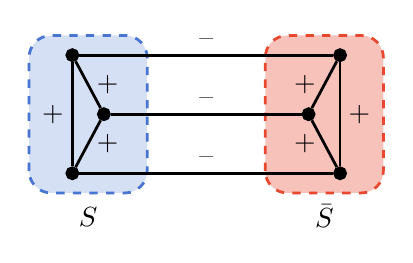
\begin{tikzpicture}[scale = 1, rounded corners=0.8em]
	\pgfsetlinewidth{1pt}
	% \tikzset{vertex/.style={circle, fill=black, minimum size=0.4em, inner sep=0.1em}};

	\filldraw[fill=c1!20, draw=c1!90, dashed] (-2.25,0) rectangle (-0.75,2);
	\filldraw[fill=c2!30, draw=c2!90, dashed] (0.75,0) rectangle (2.25,2);

	\node (X) at (-1.5, -0.3) {$S$};
	\node (Y) at (1.5, -0.3) {$\bar{S}$};

	\node[vertex] (a) at (-1.7,1.75) {};
	\node[vertex] (b) at (-1.3,1.0) {};
	\node[vertex] (c) at (-1.7,0.25) {};

	\node[vertex] (d) at (1.7,1.75) {};
	\node[vertex] (e) at (1.3,1.0) {};
	\node[vertex] (f) at (1.7,0.25) {};

	\draw (a) edge node [midway, right] {+} (b);
	\draw (a) edge node [midway, left] {+} (c);
	\draw (b) edge node [midway, right] {+} (c);
	\draw (d) edge node [midway, left] {+} (e);
	\draw (d) edge node [midway, right] {+} (f);
	\draw (e) edge node [midway, left] {+} (f);

	\draw (a) edge node [midway, above] {--} (d);
	\draw (b) edge node [midway, above] {--} (e);
	\draw (c) edge node [midway, above] {--} (f);
	% \draw (-1,1.5) -- (1,1.7) node [midway, above] {--};
	% \draw (-1,1) -- (1,0.9) node [midway, above] {--};
	% \draw (-1,0.4) -- (1,0.5) node [midway, above] {--};

\end{tikzpicture}

        \captionof{figure}{\footnotesize Grafo de sinais balanceado.}
	\end{minipage}
\end{frame}
\begin{frame}
    \begin{definition}
        Um ciclo em um grafo de sinais é chamado de \textbf{\textit{ciclo negativo}} se possuir um número \textbf{ímpar} de arestas negativas.
    \end{definition}
    % \vspace{2em}
    \begin{minipage}[h][10em][c]{\textwidth}
		\centering%
		  \begin{tikzpicture}[scale = 0.7, remember picture, overlay]
    \pgfsetlinewidth{1pt}
    % \tikzset{vertex/.style={circle, fill=black, minimum size=0.8em, inner sep=0.1em}};


	{
		\node[vertex] (c3) at (-1,1){};
	}
	{
		\node[vertex] (c7) at (1,1){};
	}
	{
		\node[vertex] (c5) at (-1,-1){};
	}
	{
		\node[vertex] (c6) at (1,-1){};
	}
    \only<2->{
        \node[vertex, text=white] (c3) at (-1,1){\tiny ?};
        \node[vertex, fill=c1, draw=c1] (c7) at (1,1){};
        \node[vertex, fill=c1, draw=c1] (c5) at (-1,-1){};
        \node[vertex, fill=c2, draw=c2] (c6) at (1,-1){};
    }
    {
        \draw (c3) edge node [label, midway, left] {--} (c5);
		\draw (c5) edge node [label, midway, below] {--} (c6);
		\draw (c6) edge node [label, midway, right] {--} (c7);
		\draw (c7) edge node [label, midway, above] {+} (c3);
	}
  \end{tikzpicture}

        \vspace{2em}
		\small{\captionof{figure}{\footnotesize Ciclo negativo.}}
	\end{minipage}
    \vspace{-2.5em}
    \pause
    \begin{theorem}[\cite{cartwright1956structural}]\label{teo:neg-cycle}
        Um grafo de sinais é balanceado se, e somente se, não possuir ciclos negativos.
    \end{theorem}
\end{frame}

\subsection{Definição do problema}
\begin{frame}
    \textsc{\textbf{\color{primary} Subgrafo Gerador Balanceado Máximo (MBSS)}}.
    \vspace{0.25em}

    {\itshape
    \noindent\textbf{Entrada:} Um grafo de sinais $G=(V,E, \sigma)$.

    \noindent\textbf{Objetivo:} Encontrar um subconjunto de arestas $E' \subseteq E$, de tamanho máximo, que gera um subgrafo balanceado.}

    \pause
    \vspace{1em}
    \begin{minipage}[h][8em][c]{\textwidth}
		\centering%
		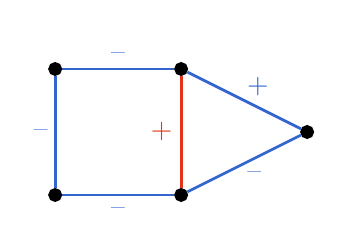
\begin{tikzpicture}[scale = 0.8]
\pgfsetlinewidth{1pt}
% \tikzset{vertex/.style={circle, fill=black, minimum size=0.8em, inner sep=0.1em, font=\tiny, text=white}};


% \node[vertex] (c1) at (-3,0){};

\node[vertex] (c2) at (-1,1){};

\node[vertex] (c3) at (-1,-1){};

\node[vertex] (c4) at (1,1){};

\node[vertex] (c5) at (3,0){};

\node[vertex] (c6) at (1,-1){};

%    \node[text=c1] (E') at (0, -1.5) {\tiny $E'=\{ab, bc, ac, cd, df, ef\}$};
% \node[text=c2] (F) at (0, -1.8) {\tiny $F = \{de\}$};

% \draw (c1) edge[c1] node [label, midway, above left] {--} (c2);
\draw (c2) edge[c1] node [label, midway, left] {--} (c3);
\draw (c2) edge[c1] node [label, midway, above] {--} (c4);
% \draw (c3) edge[c1]  node [label, midway, below] {+} (c1);
\draw (c3) edge[c1] node [label, midway, below] {--} (c6);

\draw (c4) edge[c1] node [label, midway, above right] {+} (c5);
\draw (c5) edge[c1] node [label, midway, below right] {--} (c6);
\draw (c6) edge[c2] node [label, midway, left] {+} (c4);

\end{tikzpicture}
		\small{\captionof{figure}{\footnotesize Subgrafo Gerador Balanceado Máximo \textcolor{c1}{$E'$}.}}
	\end{minipage}
    \pause

    \vspace{1em}
    {\small\alert{O problema é \textbf{NP}-Difícil, pois é generalização do \textsc{Max-Cut}.}}
\end{frame}

\section{Formulação de PI para o MBSS}
\subsection{Modelo XOR}
\begin{frame}
    \begin{block}{Modelo XOR [\cite{aref2020modeling}]}
        \begingroup
            \begin{center}
                \footnotesize
                $x_u=
                \begin{cases}
                    1, \text{\footnotesize se $u$ está na partição um}\\
                    0, \text{\footnotesize c.c}
                \end{cases}
                \text{$,\forall u \in V$}
                \;
                y_{uv}=
                \begin{cases}
                    1, \text{\footnotesize se $uv$ é removida do subgrafo gerador}\\
                    0, \text{\footnotesize c.c}
                \end{cases}
                \text{$, \forall uv \in E$}
                $
            \end{center}
            \begin{align} 
                 \min\:\:&\sum_{uv \in E} y_{uv} & & \\
                \text{s.a}:\:&x_u-x_v \leq y_{uv} &\forall uv\in E^+ \label{eq:pos1}\\
                &x_v-x_u \leq y_{uv} &\forall uv\in E^+ \label{eq:pos2}\\
                &1 - x_u - x_v \leq y_{uv} &\forall uv\in E^- \label{eq:neg1}\\
                & x_u+x_v -1 \leq y_{uv} &\forall uv\in E^- \label{eq:neg2}\\
                &x_u \in \{0,1\} &\forall u \in V\\
                &y_{uv} \in \{0,1\} &\forall uv \in E \label{eq:ybin}
            \end{align}  
        \endgroup
    \end{block}
\end{frame}

\subsection{Desigualdade de ciclos negativos}
\begin{frame}
    Seja $C^-$ o conjunto de todos os ciclos negativos em $G$, então
    \vspace{1em}
    \begin{align}
		\qquad \sum_{uv \in E(C)} y_{uv} \geq 1,\quad\forall C \in C^- \label{NEC}
	\end{align}
    é válida.

    \pause
    \vspace{1em}
    {\alert{Número possivelmente exponencial de restrições!}}
    
\end{frame}

\section{Desigualdades de cliques particionáveis}
\subsection{Definição}
\begin{frame}
    
    \begin{definition}[\cite{figueiredo2011exact}]
        Seja $K$ uma clique e $S, \bar{S} = V(K)\setminus S$. $K$ é clique particionável se:
        
        \begin{itemize}
            \item $E[S] \cup E[\bar{S}] = E^-(K)$;
            \item $[S, \bar{S}] = E^+(K)$
        \end{itemize}
    \end{definition}

    \vspace{2em}
    \begin{minipage}[h][10em][c]{\textwidth}
		\centering%
		% \input{figuras/tikz/preamble}
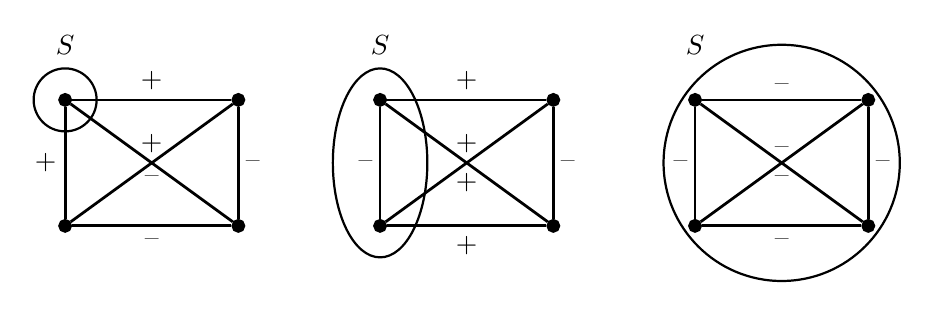
\begin{tikzpicture}
	\pgfsetlinewidth{1pt}


    \begin{scope}[shift={(-4,0)}]
    
        % Optional: draw a dotted ellipse to show partition groups
        \node[text=black] (S) at (0, 1.5) {$S$};
        \filldraw[fill=white, draw=black, thick] (0,0.8) ellipse (0.4 and 0.4);
        % \filldraw[fill=red!30, draw=red!90, dashed, rounded corners] (3,0) ellipse (1 and 1.6);
        
        % Partition A (single vertex)
        \node[vertex] (A1) at (0,0.8) {};
        \node[vertex] (A2) at (0,-0.8) {};

        \draw[draw] (A1) -- node [label, midway, left] {+} (A2);
        
        % Partition B (rest of the clique)
        \node[vertex] (B2) at (2.2,0.8) {};
        % \node[vertex] (B3) at (3,0) {};
        \node[vertex] (B4) at (2.2,-0.8) {};
        
        % Connect partition A to all B nodes
        \draw (A1) -- node [label, midway, above] {+} (B2);
        \draw (A1) -- node [label, midway, above] {+} (B4);
        
        \draw (A2) -- node [label, midway, below] {--} (B2);
        \draw (A2) -- node [label, midway, below] {--} (B4);
        
        % Connect all B nodes to each other (complete graph)
        \foreach \i/\j in {2/4} {
            \draw[draw] (B\i) -- node [label, midway, right] {--} (B\j);
        }
        
    \end{scope}

    % Picture in Quadrant II
    \begin{scope}[shift={(0,0)}]
        % Optional: draw a dotted ellipse to show partition groups
        \node[text=black] (S) at (0, 1.5) {$S$};
        \filldraw[fill=white, draw=black, thick] (0,0) ellipse (0.6 and 1.2);
        % \filldraw[fill=red!30, draw=red!90, dashed, rounded corners] (3,0) ellipse (1 and 1.6);
        
        % Partition A (single vertex)
        \node[vertex] (A1) at (0,0.8) {};
        \node[vertex] (A2) at (0,-0.8) {};

        \draw[draw] (A1) -- node [label, midway, left] {--} (A2);
        
        % Partition B (rest of the clique)
        \node[vertex] (B2) at (2.2,0.8) {};
        % \node[vertex] (B3) at (3,0) {};
        \node[vertex] (B4) at (2.2,-0.8) {};
        
        % Connect partition A to all B nodes
        \draw (A1) -- node [label, midway, above] {+} (B2);
        \draw (A1) -- node [label, midway, above] {+} (B4);
        
        \draw (A2) -- node [label, midway, below] {+} (B2);
        \draw (A2) -- node [label, midway, below] {+} (B4);
        
        % Connect all B nodes to each other (complete graph)
        \foreach \i/\j in {2/4} {
            \draw[draw] (B\i) -- node [label, midway, right] {--} (B\j);
        }
    \end{scope}

    % Picture in Quadrant II
    \begin{scope}[shift={(4,0)}]
        % Optional: draw a dotted ellipse to show partition groups
        \node[text=black] (S) at (0, 1.5) {$S$};
        \filldraw[fill=white, draw=black, thick] (1.1,0) ellipse (1.5 and 1.5);
        % \filldraw[fill=red!30, draw=red!90, dashed, rounded corners] (3,0) ellipse (1 and 1.6);
        
        % Partition A (single vertex)
        \node[vertex] (A1) at (0,0.8) {};
        \node[vertex] (A2) at (0,-0.8) {};

        \draw[draw] (A1) -- node [label, midway, left] {--} (A2);
        
        % Partition B (rest of the clique)
        \node[vertex] (B2) at (2.2,0.8) {};
        % \node[vertex] (B3) at (3,0) {};
        \node[vertex] (B4) at (2.2,-0.8) {};
        
        % Connect partition A to all B nodes
        \draw (A1) -- node [label, midway, above] {--} (B2);
        \draw (A1) -- node [label, midway, above] {--} (B4);
        
        \draw (A2) -- node [label, midway, below] {--} (B2);
        \draw (A2) -- node [label, midway, below] {--} (B4);
        
        % Connect all B nodes to each other (complete graph)
        \foreach \i/\j in {2/4} {
            \draw[draw] (B\i) -- node [label, midway, right] {--} (B\j);
        }
    \end{scope}
    
    
\end{tikzpicture}
        \vspace{1em}
		\small{\captionof{figure}{\footnotesize Cliques particionáveis.}}
	\end{minipage}
    
\end{frame}


\section{Desigualdades de cliques particionáveis}
\subsection{Desigualdades}
\begin{frame}

    \begin{itemize}
        \item Inspiração em: An exact approach to the problem of extracting an embedded network matrix [\cite{figueiredo2011exact}];
        \item Auxílio do software PORTA.
    \end{itemize}

    \pause
    \begin{theorem}
        Seja $K$ uma clique particionável em partições $S$ e $\bar S=V(K)\setminus S$, com $k=|V(K)|$. A desigualdade:
        \begin{equation}\label{eq:ineq2}
            -(k-3)\sum_{u \in S}x_u + (k-3)\sum_{v \in \bar{S}}x_v + \sum_{e \in E(K)}y_e \geq \frac{(k-1)(k-2)}{2} + (k-3)(1- |S|)
        \end{equation}
        é válida para $k \geq 2$
    \end{theorem}

    \pause
    
    \vspace{1em}
    {\alert{Induz faceta no politopo da formulação XOR!}}
    
\end{frame}

\subsection{Exemplo}
\begin{frame}
    
Exemplo: $k=4$.

\begin{itemize}
    \item $S = V(K), \bar{S} = \emptyset$: 
        \begin{equation}
            {\only<2>{\color{c1}}-\sum_{u \in V(K)}x_u} + {\only<2>{\color{c2}} \sum_{e \in E(K)}y_e} \geq 0 
        \end{equation}
    \item $S = \emptyset, \bar{S} = V(K)$:
        \begin{equation}
            {\only<2>{\color{c1}}\sum_{u \in V(K)}x_u} + {\only<2>{\color{c2}} \sum_{e \in E(K)}y_e} \geq 4
        \end{equation}
\end{itemize}

\begin{minipage}[h][10em][c]{\textwidth}
    \centering%
    \input{figures/ex-clique negativa.tex}
    \captionof{figure}{\footnotesize Clique negativa.}
\end{minipage}

\end{frame}

\section{Experimentos computacionais}

\subsection{Algoritmo branch-and-cut}

\begin{frame}
    
    Versão base: restrições XOR, fixando em 1 o valor da variável $x$ do vértice de maior grau. \\[1em]

    \pause
    
    \begin{enumerate}
        \item \textbf{NC}: Desigualdades de ciclos negativos disjuntos em arestas (priorizando triângulos);
        \pause
        \item \textbf{TRI}: Desigualdades de triângulos negativos como cortes adicionados pelo \textit{solver};
        \pause
        \item \textbf{K4}: Desigualdades de cliques particionáveis (tam. 4), seguindo os parâmetros $\epsilon, r, \kappa$;
        \pause
        \item \textbf{H}: Heurística de \cite{iacono2010determining} para fornecer uma solução inicial. 
    \end{enumerate}
    
\end{frame}

\subsection{Ambiente e instâncias}

\begin{frame}

    \begin{block}{Ambiente computacional}
        \begin{itemize}
            \item AMD Ryzen 5 5700G, 22 GB de RAM e S.O. Ubuntu 24.04 LTS;
            \item Linguagem C++ e \textit{solver} \textit{IBM ILOG CPLEX 22.1.1};
            \item Tamanho máximo da árvore B\&C = 20 GB;
            \item Tempo máximo de execução do \textit{solver} = 1 hora.
        \end{itemize}
    \end{block}

    \begin{block}{Instâncias}
        \begin{itemize}
            \item Instâncias aleatórias com parâmetros $n \in \{100,200\}$, $d \in \{30\%, 50\%, 70\%\}$, $p \in \{25\%, 50\%, 75\%\}$.
        \end{itemize}       
    \end{block}
    
\end{frame}

\subsection{Resultados}

\begin{frame}

    \begin{figure}[h]
        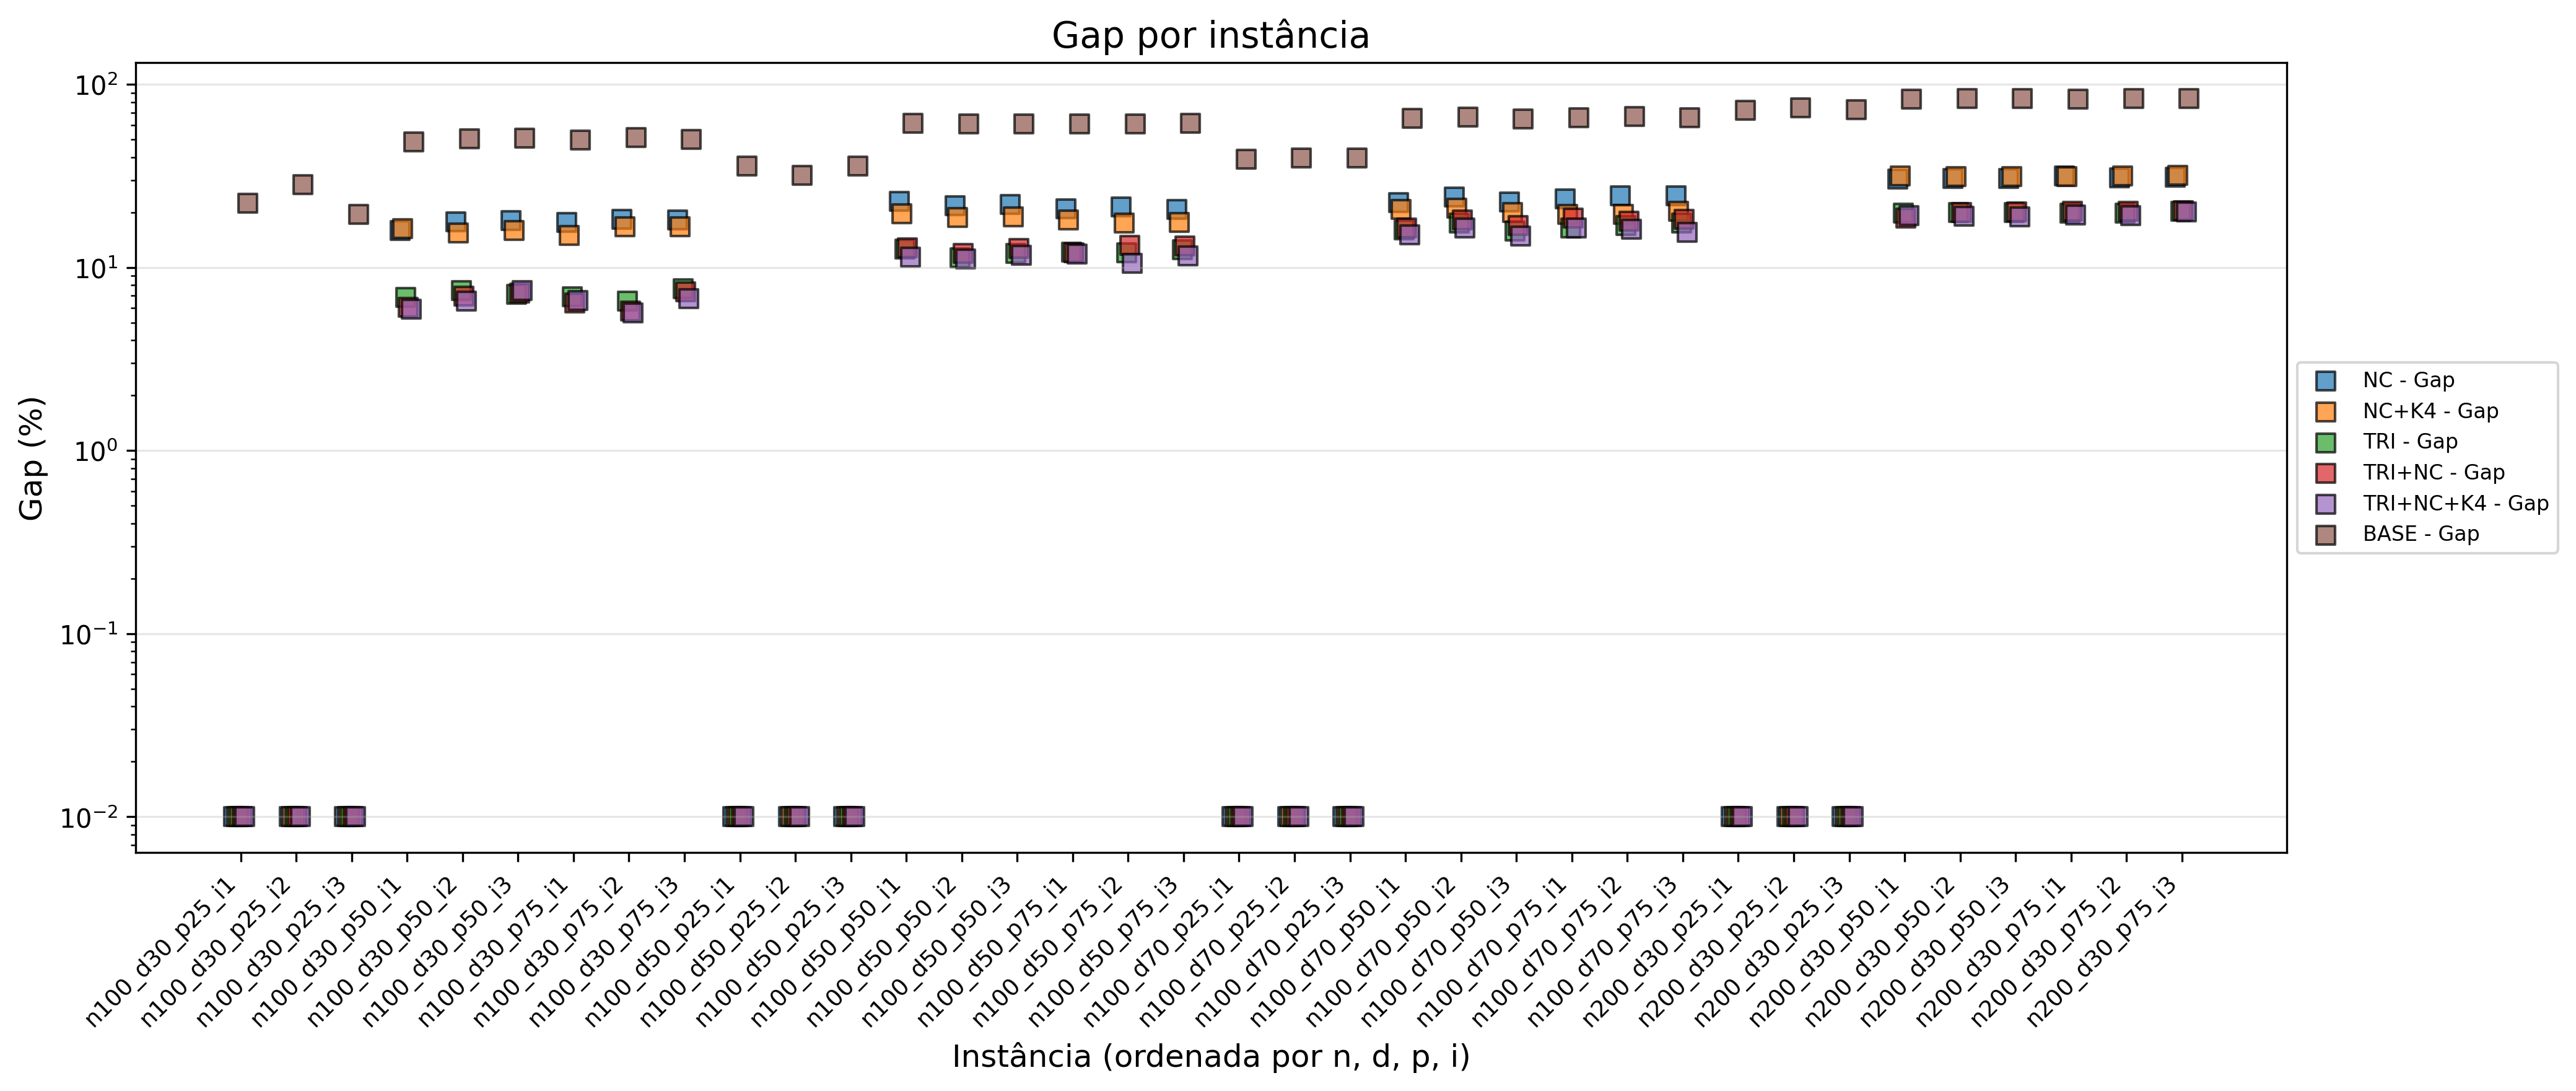
\includegraphics[width=\textwidth]{figures/grafico_gaps_por_instancia.png}
        \captionof{figure}{Resultados das instâncias de 100 e 200 vértices.}
        \label{fig:figure2}
    \end{figure}
    
\end{frame}

\begin{frame}
\begin{table}[h]
\scriptsize
% \renewcommand{\arraystretch}{0.9}
% \setlength{\tabcolsep}{4pt}
\label{tab:sint-200}
\centering
\begin{tabular}{l|l|rr|rr|rr|rr|rr|rr}
\hline
\multirow{2}{*}{$(n,d,p)$} & \multirow{2}{*}{i} & \multicolumn{2}{c|}{BASE+H} & \multicolumn{2}{c|}{NC+H} & \multicolumn{2}{c|}{NC+K4+H} & \multicolumn{2}{c|}{TRI+H} & \multicolumn{2}{c|}{TRI+NC+H} & \multicolumn{2}{c}{TRI+NC+K4+H} \\
&  & Tempo & Gap & Tempo & Gap & Tempo & Gap & Tempo & Gap & Tempo & Gap \\
\hline
& 1 & TL & 73,23 & 11,39 & -- & 79,76 & -- & 6,46 & -- & \textbf{1,79} & -- & 2,29 & -- \\
(200, 50\%, 25\%) & 2 & TL & 73,86 & 9,54 & -- & 75,17 & -- & 7,96 & -- & \textbf{1,63} & -- & 1,85 & -- \\
& 3 & TL & 74,29 & 12,92 & -- & 160,77 & -- & 8,53 & -- & \textbf{1,71} & -- & 2,56 & -- \\
\hline
& 1 & TL & 85,97 &TL & 29,17 & TL & 30,31 & TL & 23,31 & TL & 23,31 & TL & \textbf{22,72} \\
(200, 50\%, 50\%) & 2 & TL & 86,05& TL & 28,32 & TL & 29,17 & TL & 22,05 & TL & 22,05 & TL & \textbf{21,47} \\
& 3 & TL & 86,08 & TL & 28,55 & TL & 29,61 & TL & 22,66 & TL & 22,66 & TL & \textbf{22,02} \\
\hline
& 1 & TL & 86,98 & TL & 29,31 & TL & 29,16 & TL & 23,21 & TL & 23,21 & TL & \textbf{22,64} \\
(200, 50\%, 75\%) & 2 & TL & 87,32 & TL & 29,44 & TL & 29,49 & TL & 23,60 & TL & 23,62 & TL & \textbf{23,09} \\
& 3 & TL & 86,11 & TL & 28,91 & TL & 28,68 & TL & 22,77 & TL & 22,77 & TL & \textbf{22,20} \\
\hline
& 1 & TL & 76,96 & 16,93 & -- & 358,67 & -- & 18,83 & -- & \textbf{3,08} & -- & 5,24 & -- \\
(200, 70\%, 25\%) & 2 & TL & 76,96 & 15,38 & -- & 272,03 & -- & 17,67 & -- & \textbf{3,30} & -- & 5,20 & -- \\
& 3 & TL & 77,28 & 21,13 & -- & 315,12 & -- & 19,48 & -- & \textbf{3,08} & -- & 6,19 & -- \\
\hline
& 1 & TL & 87,93 & TL & 28,86 & TL & 29,61 & TL & \textbf{24,32} & TL & 24,32 & TL & 26,96 \\
(200, 70\%, 50\%) & 2 & TL & 88,11 & TL & 28,89 & TL & 29,56 & TL & 24,88 & TL & \textbf{24,59} & TL & 27,23 \\
& 3 & TL & 87,89 & TL & 28,07 & TL & 28,76 & TL & \textbf{23,79} & TL & 26,05 & TL & 26,41 \\
\hline
& 1 & TL & 87,95 & TL & 29,04 & TL & 29,60 & TL & 25,00 & TL & \textbf{24,76} & TL & 27,35 \\
(200, 70\%, 75\%) & 2 & TL & 88,12 & TL & 29,20 & TL & 29,87 & TL & 25,03 & TL & \textbf{24,82} & TL & 27,51 \\
& 3 & TL & 88,04 & TL & 29,35 & TL & 30,10 & TL & 25,94 & TL & \textbf{25,07} & TL & 27,59 \\
\hline
\end{tabular}
\caption{Resultados para instâncias sintéticas com 200 vértices, utilizando a heurística.}
\end{table}    
\end{frame}

\begin{frame}
    \begin{table}[h]
    \label{tab:sint-200.2}
    \centering
    \begin{tabular}{l|l|rr}
        \hline
        \multirow{2}{*}{$(n,d,p)$} & \multirow{2}{*}{i} & \multicolumn{2}{c}{TRI+NC+K4+H} \\
        &  & Tempo & Gap \\
        \hline
        & 1 & TL & \textbf{24,27} \\
        (200, 70\%, 50\%) & 2 & TL & 26,95 \\
        & 3 & TL & \textbf{25,99} \\
        \hline
        & 1 & TL & 27,28 \\
        (200, 70\%, 75\%) & 2 & TL & \textbf{24,80} \\
        & 3 & TL & \textbf{24,85} \\
        \hline
    \end{tabular}
    \caption{Resultados para instâncias com 200 vértices com outros parâmetros para K4.}
    \end{table}
\end{frame}

\section{}

\begin{frame}{}{}
    \vfill
    \begin{center}
    {\Large Obrigada!}
    \end{center}

    \vfill

    \begin{figure}
    \centering
    
\includegraphics[height=1.5cm]{figures/logopqno.png}\hspace{1cm}
    
\includegraphics[height=0.7cm]{figures/mdcc-cabecalho.png}\hspace{1cm}
    
\includegraphics[height=0.7cm]{figures/pargo.png}\hspace{1cm}
    
\includegraphics[height=0.7cm]{figures/funcap.png}\hspace{1cm}
    
\includegraphics[height=1.5cm]{figures/cnpq.png}
    \end{figure}
\end{frame}

\begin{frame}[allowframebreaks]{Referências}
    \printbibliography
\end{frame}

\begin{frame}

    \begin{figure}[h]
        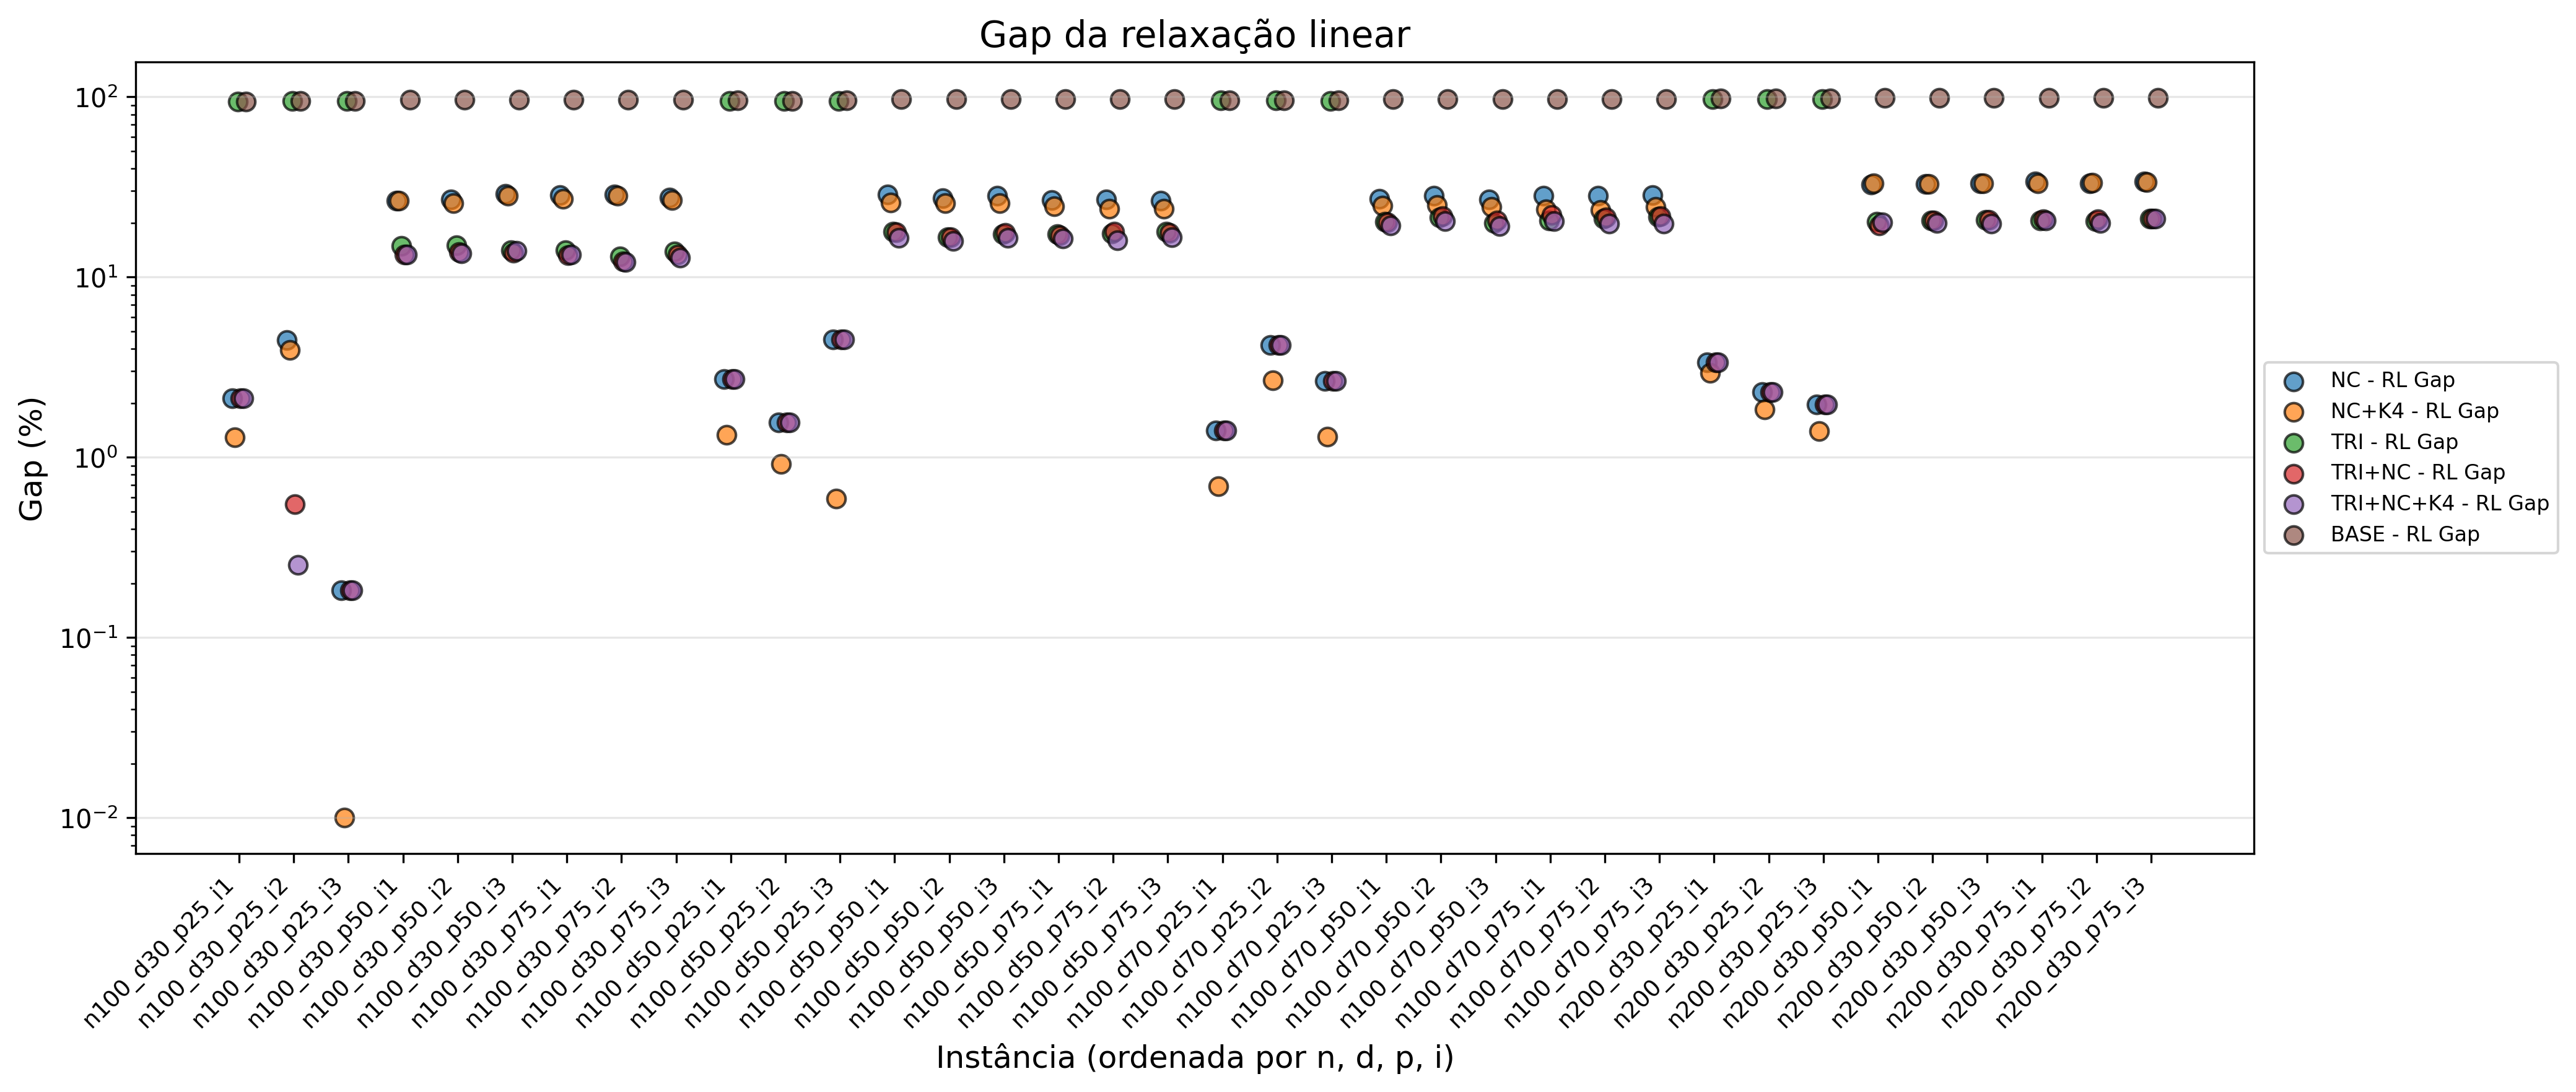
\includegraphics[width=\textwidth]{figures/gap_relaxacao.png}
        \captionof{figure}{Resultados das instâncias de 100 e 200 vértices.}
        \label{fig:figure2}
    \end{figure}
    
\end{frame}

\begin{frame}[allowframebreaks] 
    
    {\scriptsize
    \renewcommand{\arraystretch}{0.9}  % valores < 1 diminuem o espaço
    \setlength{\tabcolsep}{3pt}  % padrão é 6pt
    \begin{longtable}{l|c|rr|rr|rr|rr|rr|rr}
    \caption{Resultados para instâncias sintéticas com 100 e 200 vértices.}
    \label{tab:sint-100-200}\\
    \hline
    \multirow{2}{*}{$(n,d,p)$} & \multirow{2}{*}{i} & \multicolumn{2}{c|}{BASE} & \multicolumn{2}{c|}{NC} & \multicolumn{2}{c|}{NC+K4} & \multicolumn{2}{c|}{TRI} & \multicolumn{2}{c|}{TRI+NC} & \multicolumn{2}{c}{TRI+NC+K4} \\
    & &Tempo & Gap  & Tempo & Gap & Tempo & Gap & Tempo & Gap & Tempo & Gap & Tempo & Gap \\
    \hline
    \endfirsthead

    \multicolumn{14}{c}%
    {\tablename\ \thetable\ -- continuação da página anterior} \\
    \hline
    \multirow{2}{*}{$(n,d,p)$} & \multirow{2}{*}{i} & \multicolumn{2}{c|}{BASE} & \multicolumn{2}{c|}{NC} & \multicolumn{2}{c|}{NC+K4} & \multicolumn{2}{c|}{TRI} & \multicolumn{2}{c|}{TRI+NC} & \multicolumn{2}{c}{TRI+NC+K4} \\
    & & Tempo & Gap & Tempo & Gap & Tempo & Gap & Tempo & Gap & Tempo & Gap & Tempo & Gap \\
    \hline
    \endhead

    \hline
    \multicolumn{14}{r}{continua na próxima página} \\
    \endfoot

    \hline
    \endlastfoot
    & 1 & TL & 22,37 & 0,10 & -- & 0,22 & -- & 0,13 & -- & \textbf{0,07} & -- & 0,08 & -- \\
    (100, 30\%, 25\%) & 2 & TL & 28,23 & 0,96 & -- & 1,60 & -- & \textbf{0,14} & -- & 0,17 & -- & 0,23 & -- \\
    & 3 & TL & 19,47 & \textbf{0,03} & -- & 0,12 & -- & 0,07 & -- & 0,07 & -- & 0,07 & -- \\
    \hline
    & 1 & TL & 45,57 & TM & 15,87 & TL & 15,67 & TL & 6,84 & TL & 6,05 & TL & \textbf{5,93} \\
    (100, 30\%, 50\%) & 2 & TL & 50,46 & TM & 17,71 & TL & 15,44 & TL & 7,48 & TL & 6,95 & TL & \textbf{6,55} \\
    & 3 & TL & 50,88 & TM & 18,01 & TL & 15,95 & TL & \textbf{7,15} & TL & 7,26 & TL & 7,51 \\
    \hline
    & 1 & TL & 49,81 & TM & 17,68 & TL & 14,94 & TL & 6,91 & TL & \textbf{6,39} & TL & 6,58 \\
    (100, 30\%, 75\%) & 2 & TL & 51,27 & TM & 18,25 & TL & 16,73 & TL & 6,54 & TL & 5,80 & TL & \textbf{5,65} \\
    & 3 & TL & 50,09 & TM & 18,11 & TL & 16,70 & TL & 7,68 & TL & 7,38 & TL & \textbf{6,78} \\
    \hline
    & 1 & TL & 25,76 & 0,29 & -- & 1,07 & -- & \textbf{0,06} & -- & 0,13 & -- & 0,18 & -- \\
    (100, 50\%, 25\%) & 2 & TL & 31,85 & 0,12 & -- & 1,04 & -- & \textbf{0,08} & -- & 0,10 & -- & 0,12 & -- \\
    & 3 & TL & 35,70 & 0,59 & -- & 1,68 & -- & \textbf{0,11} & -- & 0,17 & -- & 0,19 & -- \\
    \hline
    & 1 & TL & 61,04 & TM & 23,01 & TL & 19,63 & TL & 12,64 & TL & 12,82 & TL & \textbf{11,35} \\
    (100, 50\%, 50\%) & 2 & TL & 60,79 &TL & 21,73 & TL & 18,78 & TL & 11,31 & TL & 11,93 & TL & \textbf{11,09} \\
    & 3 & TL & 60,76 & TL & 22,08 & TL & 18,83 & TL & 11,91 & TL & 12,68 & TL & \textbf{11,63} \\
    \hline
    & 1 & TL & 60,73 & TM & 20,90 & TL & 18,22 & TL & 12,09 & TL & 12,04 & TL & \textbf{11,86} \\
    (100, 50\%, 75\%) & 2 & TL & 60,90 & TM & 21,43 & TL & 17,53 & TL & 12,01 & TL & 13,23 & TL & \textbf{10,54} \\
    & 3 & TL & 61,27 & TM & 20,78 & TL & 17,55 & TL & 12,47 & TL & 13,05 & TL & \textbf{11,52} \\
    \hline
    & 1 & TL & 38,89 & 0,22 & -- & 1,64 & -- & \textbf{0,12} & -- & 0,16 & -- & 0,30 & -- \\
    (100, 70\%, 25\%) & 2 & TL & 39,50 &0,80 & -- & 3,65 & -- & \textbf{0,12} & -- & 0,26 & -- & 0,42 & -- \\
    & 3 & TL & 39,52 & 0,45 & -- & 2,40 & -- & \textbf{0,13} & -- & 0,23 & -- & 0,41 & -- \\
    \hline
    & 1 &TL & 65,42 & TL & 22,68 & TL & 20,72 & TL & 16,09 & TL & 16,43 & TL & \textbf{15,10} \\
    (100, 70\%, 50\%) & 2 & TL & 66,25 &TM & 24,25 & TL & 21,14 & TL & 17,43 & TL & 18,20 & TL & \textbf{16,41} \\
    & 3 & TL & 64,86 & TL & 22,74 & TL & 20,01 & TL & 15,74 & TL & 16,99 & TL & \textbf{14,86} \\
    \hline
    & 1 & TL & 65,57 &TL & 23,73 & TL & 19,51 & TL & 16,44 & TL & 18,54 & TL & \textbf{16,38} \\
    (100, 70\%, 75\%) & 2 & TL & 66,50 &TM & 24,65 & TL & 19,45 & TL & 16,98 & TL & 17,94 & TL & \textbf{16,14} \\
    & 3 & TL & 65,60 &TM & 24,56 & TL & 20,29 & TL & 17,41 & TL & 18,29 & TL & \textbf{15,54} \\
    \hline
    & 1 & TL & 72,00 & 9,22 & -- & 50,06 & -- & \textbf{0,70} & -- & 0,95 & -- & 1,34 & -- \\
    (200, 30\%, 25\%) & 2 & TL & 74,52 & 3,53 & -- & 16,76 & -- & \textbf{0,58} & -- & 0,78 & -- & 0,88 & -- \\
    & 3 & TL & 72,65 & 2,85 & -- & 52,00 & -- & 0,81 & -- & \textbf{0,71} & -- & 0,91 & -- \\
    \hline
    & 1 & TL & 83,11 &TL & 30,36 & TL & 31,62 & TL & 19,84 & TL & \textbf{18,58} & TL & 19,20 \\
    (200, 30\%, 50\%) & 2 & TL & 83,34 & TL & 30,66 & TL & 31,24 & TL & 19,98 & TL & 20,01 & TL & \textbf{18,99} \\
    & 3 & TL & 83,61 & TM & 30,72 & TL & 31,44 & TL & 19,96 & TL & 20,09 & TL & \textbf{18,93} \\
    \hline
    & 1 & TL & 83,21 & TL & 31,67 & TL & 31,40 & TL & 19,74 & TL & 20,19 & TL & \textbf{19,41} \\
    (200, 30\%, 75\%) & 2 & TL & 83,60 &TL & 30,78 & TL & 31,47 & TL & 19,80 & TL & 20,29 & TL & \textbf{19,13} \\
    & 3 & TL & 83,61 & TL & 31,19 & TL & 31,72 & TL & 20,28 & TL & 20,48 & TL & \textbf{20,17} \\
    \end{longtable}
    }
\end{frame}

\end{document}